% !TeX spellcheck = it_IT
\newpage
\section{Business models}
Il \textbf{business model} descrive l'idea di come un'organizzazione crea, consegna e cattura del \textbf{valore}.
\subsection{Canvas}
Il Business Model Canvas è un linguaggio condiviso per descrivere, visualizzare, valutare e modificare modelli di business. Si struttura come segue:
\begin{center}
	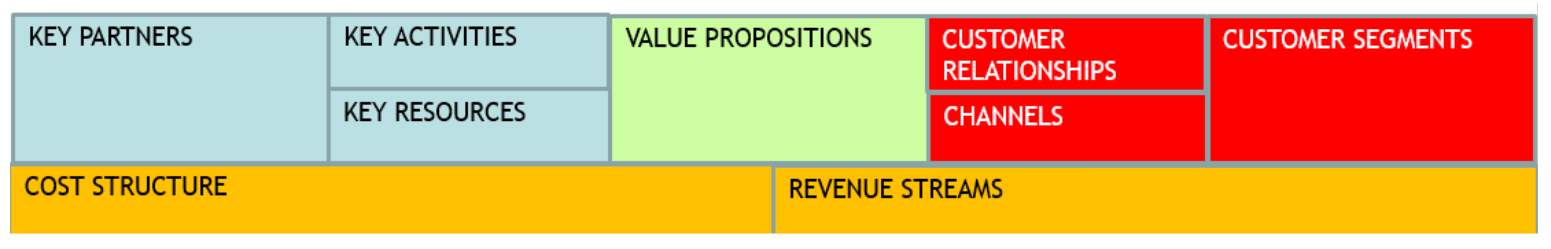
\includegraphics[scale=0.25]{business_model_canvas.png}
\end{center}
Vediamo nel dettaglio ogni sezione:
\begin{itemize}
	\item \textbf{Value propositions}: descrive l'insieme di prodotti e servizi che creano valore per un segmento specifico di clienti
	\item \textbf{Customer}
	\begin{itemize}
		\item \textbf{Segments}: definisce i diversi gruppi di persone o organizzazioni che un'impresa vuole raggiungere e servire
		\item \textbf{Relationship}: descrive i tipi di relazioni che un'azienda stabilisce con determinati segmenti
		\item \textbf{Channels}: descrive come l'azienda comunica e raggiunge i segmenti
	\end{itemize}
	\item \textbf{Key}
	\begin{itemize}
		\item \textbf{Resources}: le risorse più importanti per far funzionare un business model
		\item \textbf{Activities}: le attività più importanti per far funzionare un business model
		\item \textbf{Partners}: la rete di fornitori e partner che fanno funzionare un business model
	\end{itemize}
	\item \textbf{Revenue streams}: il guadagno di un'azienda diviso per ogni segmento
	\item \textbf{Cost structure}: tutti i costi strutturali previsti dal business model
\end{itemize}

\begin{example}[Nespresso]
	Nel 1976 la \textit{Nestré} dominava il mercato con il caffè istantaneo tramite il prodotto Nescafé. \\
	Nel 1988 la Nespresso riesce a ribaltare la situazione concentrandosi su segmenti di mercato di elite. In particolare, usa il seguente canvas:
	\begin{center}
		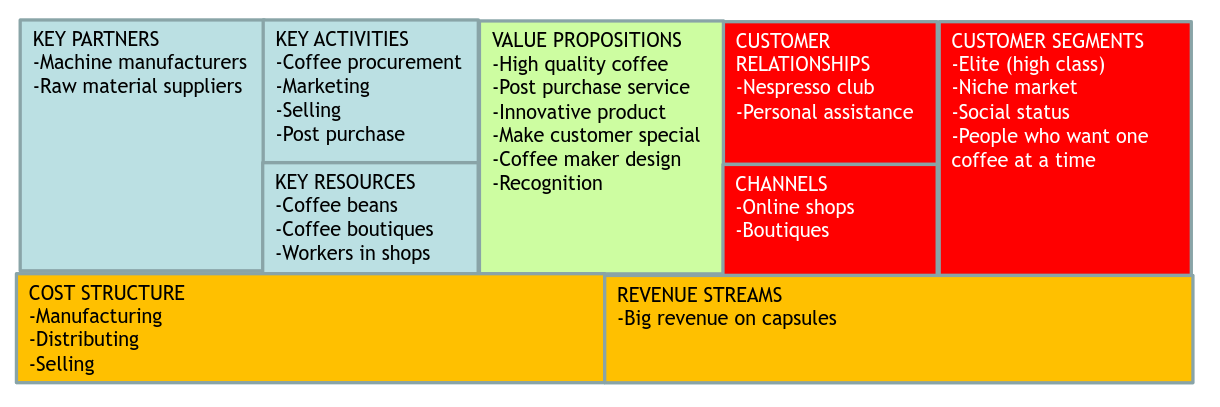
\includegraphics[scale=0.35]{nespresso_canvas.png}
	\end{center}
\end{example}

\newpage
\begin{example}[Netflix]
	Netflix è riuscito a spodestare il dominio di aziende come Blockbuster introducendo lo streaming. Vediamo il confronto tra i due canvas:
	\begin{center}
		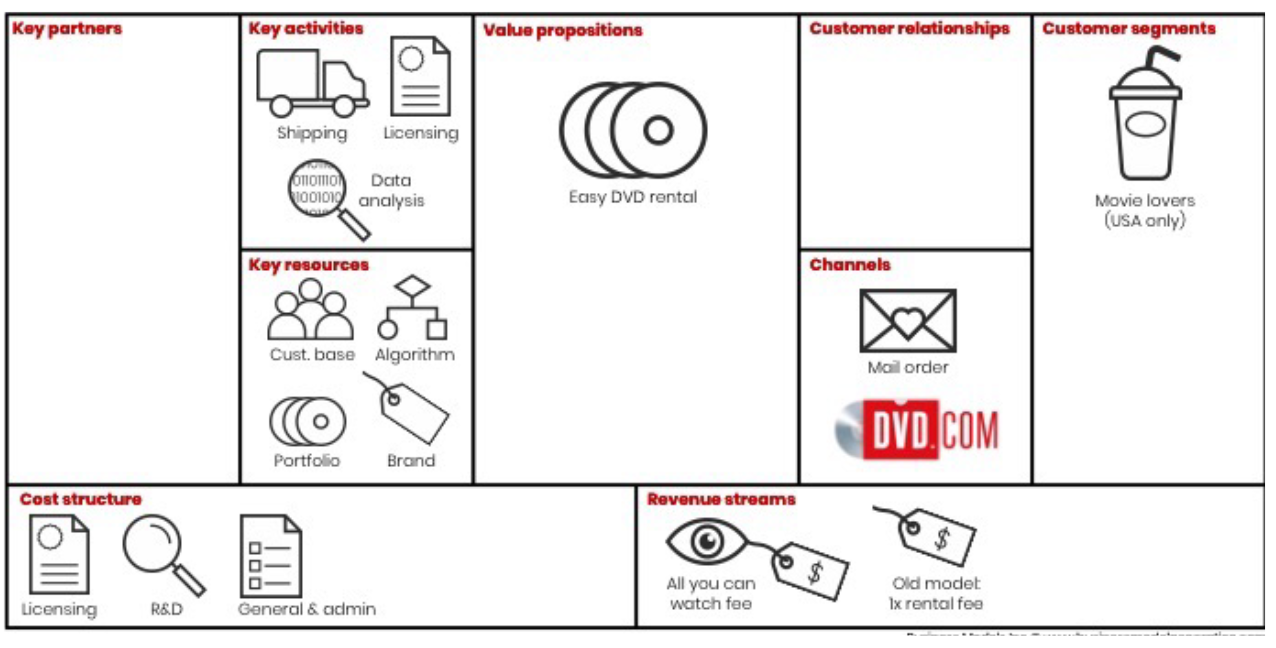
\includegraphics[scale=0.17]{blockbuster.png}
		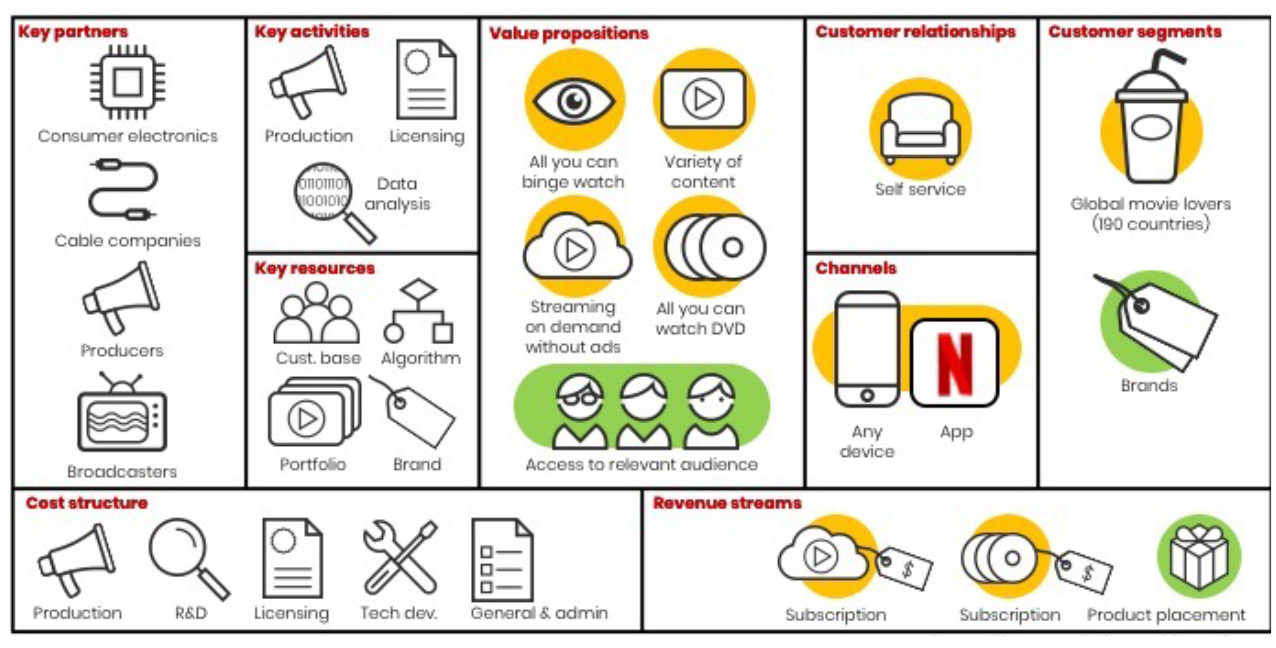
\includegraphics[scale=0.17]{netflix.png}
	\end{center}
\end{example}

\subsection{Freemium}
L'idea è di combinare funzionalità di base gratuite con servizi più avanzati a pagamento, tenendo d'occhio quanto costa all'azienda mantenere i servizi gratuiti e a che rateo gli utenti diventano premium.\\
In media il $10\%$ di tutti gli utenti diventano premium.

\begin{example}[Spotify]
	Spotify ha gli utenti gratuiti che fanno guadagnare tramite le pubblicità e quelli a pagamento che pagano l'abbonamento. Spotify deve poi pagare le commissioni a chi detiene i diritti sulla musica.
	\begin{center}
		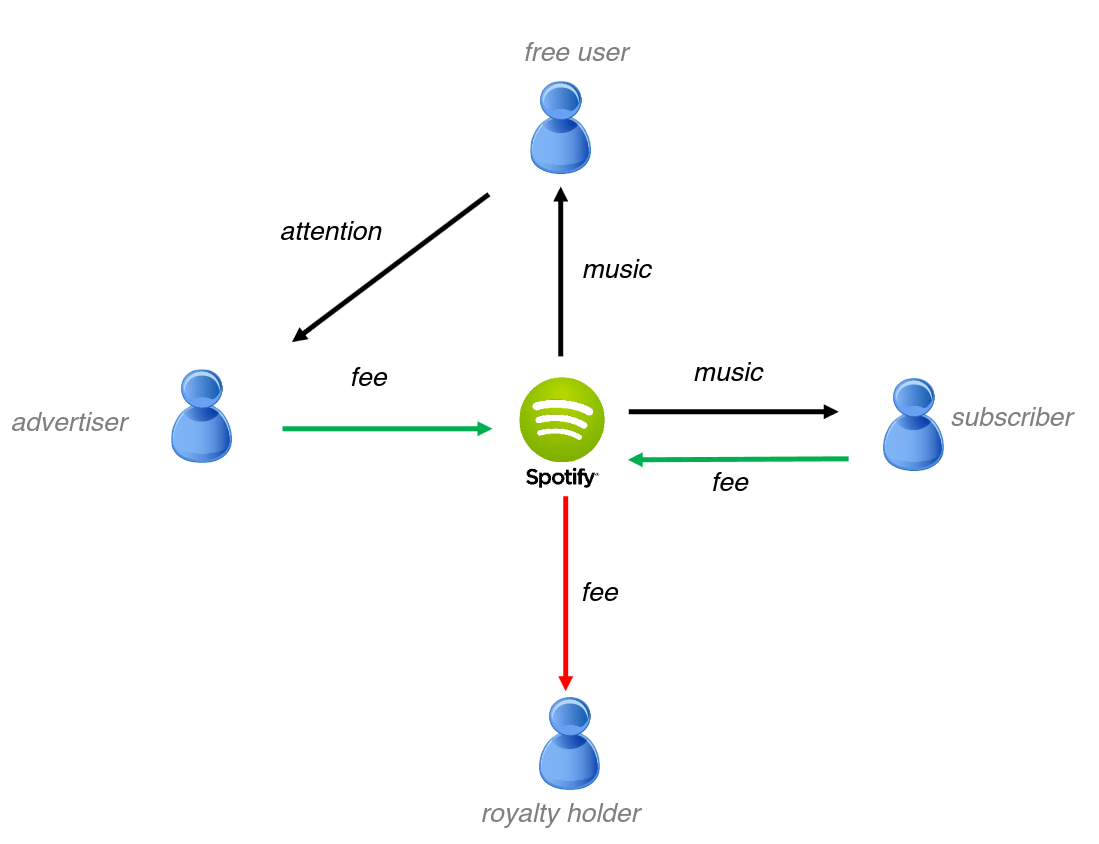
\includegraphics[scale=0.3]{spotify.png}
	\end{center}
\end{example}
\newpage
\begin{example}[Flickr]
	Vediamo il canvas di Flickr:
	\begin{center}
		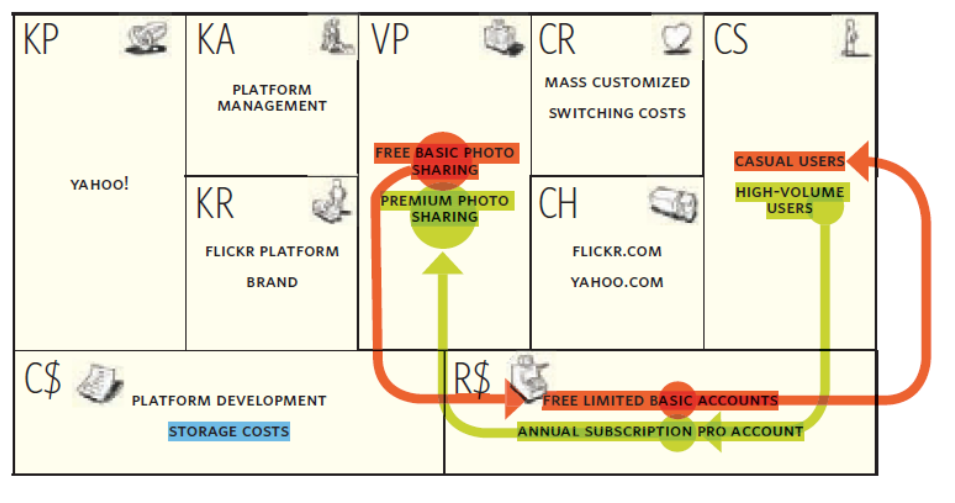
\includegraphics[scale=0.3]{flickr.png}
	\end{center}
	Anche Flickr si basa su un principio \textit{freemium}: in \color{red}rosso \color{black} il tier gratuito mentre in \color{green}verde \color{black} quello a pagamento.
\end{example}

\begin{example}[Redhat]
	Redhat si concentra sul segmento di mercato delle aziende che vogliono sfruttare prodotti opensource ma che vogliono anche che ci sia qualcuno di responsabile (anche legalmente).
	\begin{center}
		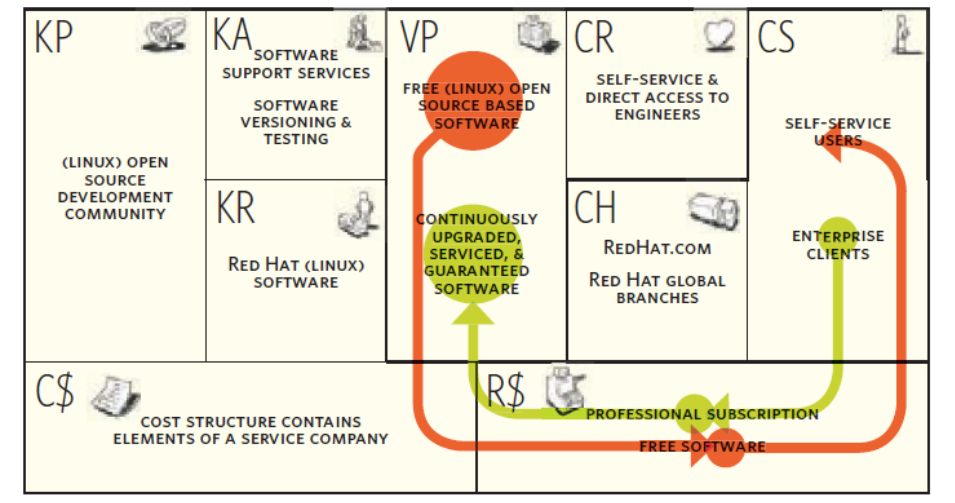
\includegraphics[scale=0.3]{redhat.png}
	\end{center}
\end{example}

\begin{example}[Skype]
	Permette di fare chiamate gratuite attraverso internet.
	\begin{center}
		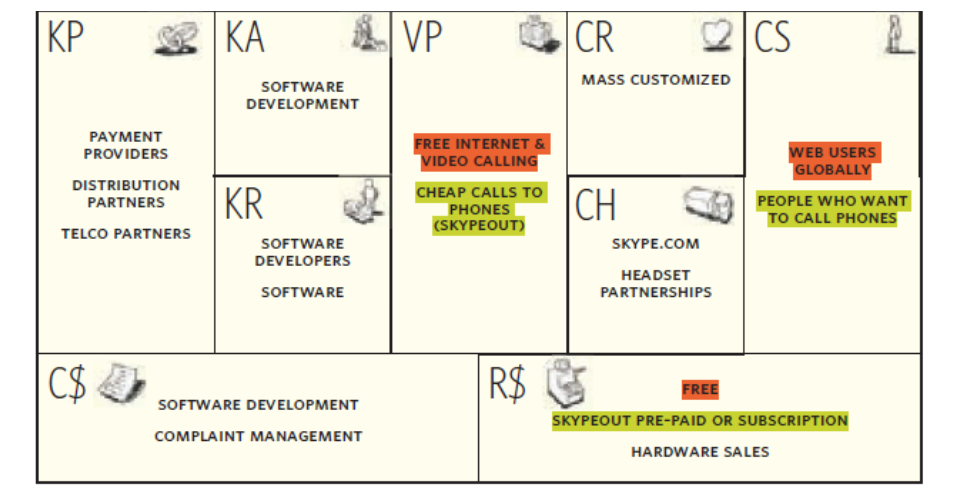
\includegraphics[scale=0.3]{skype.png}
	\end{center}
\end{example}

\begin{note}
	Anche Dropbox utilizza un principio freemium. A differenza di Netflix, Dropbox si è poi distaccato da Amazon AWS e ha creato la sua infrastruttura.
\end{note}

\newpage
\subsection{Innovazione}
L'innovazione parte dal cambio di prospettiva: bisogna concentrarsi su quella del cliente. Da qui poi possiamo farci le domande \textbf{what if...?}, che ci portano ad identificare principalmente quattro epicentri di miglioramento:
\begin{itemize}
	\item \textbf{Resource Driven}: queste innovazioni nascono da un'infrastruttura preesistente per \textit{espandere} o \textit{trasformare} il business model. Un esempio è Amazon AWS.
	\item \textbf{Customer Driven}: queste innovazioni si basano sulle \textit{necessità del cliente}, sulla \textit{facilità di accesso} o sul migliorare la \textit{comodità}. Influenza delle parti specifiche del business model. Un esempio è 23andMe che offre test del DNA specifici per certe richieste.
	\item \textbf{Offer Driven}: le innovazioni di questo tipo creano una nuova \textit{value proposition}, ad esempio Cemex consegna il cemento in 4 ore invece che 48.
	\item \textbf{Finance Driven}: innovazioni che \textit{riducono i costi} o \textit{aumentano i guadagni} (anche introducendo nuove fonti). Un esempio è Xerox che fornisce le prime 2000 copie gratuite.
\end{itemize}

\subsection{Casi di studio}
\subsubsection{Amazon}
Amazon (originariamente \textit{Cadabra}) viene fondata da Jeff Bezos nel 1994 come negozio online di libri. Non si aspettava di avere profitti per i primi 4 o 5 anni e infatti il primo quadrimestre positivo è stato l'ultimo del 2001.\\
Al 2022 i guadagni (in miliardi di dollari) si dividono in:
\begin{enumerate}
	\item $231.87$ dallo store online
	\item $140.05$ dai servizi ai venditori di terze parti
	\item $90.76$ da AWS
	\item $40.20$ da abbonamenti (e.g. Prime)
	\item $20.03$ da negozi fisici
\end{enumerate}
\subsubsection{Google}
I guadagni di Google si concentrano sulle \textbf{pubblicità personalizzate}:
\begin{center}
	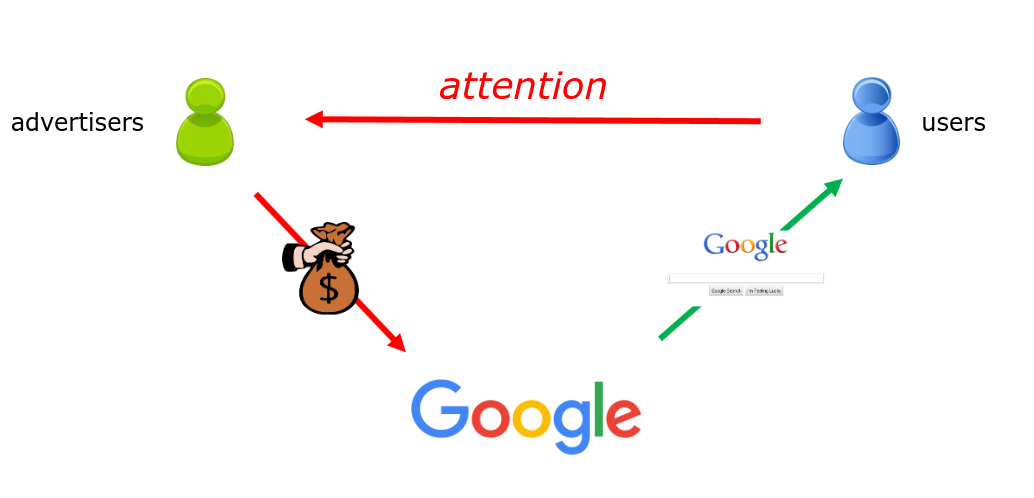
\includegraphics[scale=0.3]{google.png}
\end{center}
non solo tramite il motore di ricerca ma anche con tutte le altre applicazioni che forniscono.